% Created by tikzDevice version 0.7.0 on 2015-01-10 18:42:08
% !TEX encoding = UTF-8 Unicode
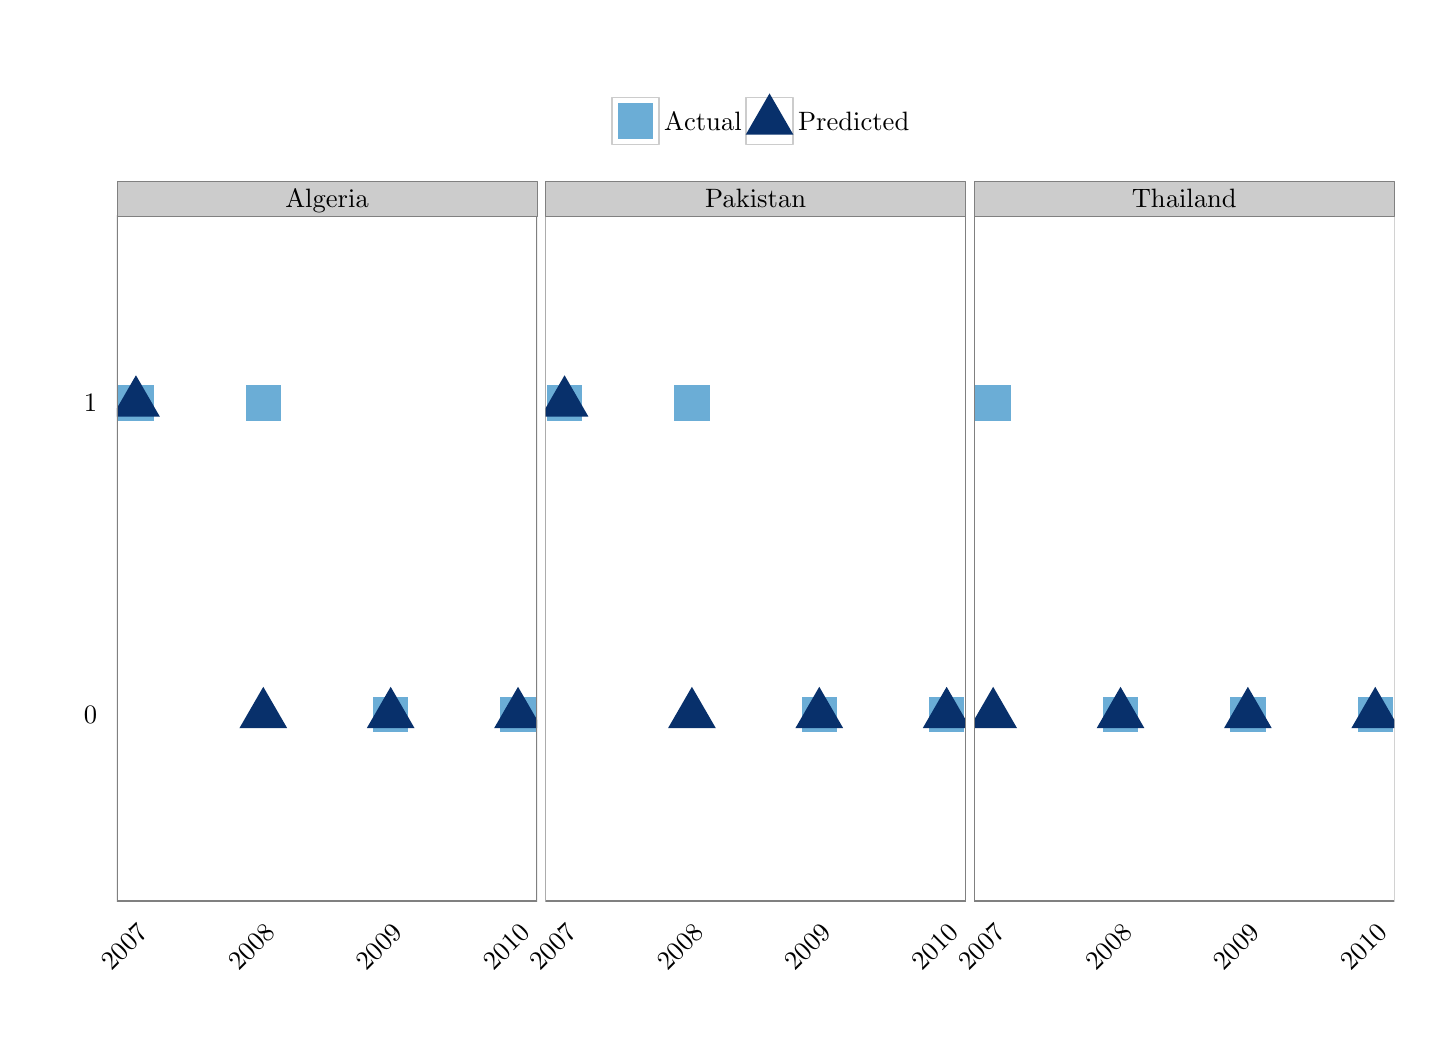
\begin{tikzpicture}[x=1pt,y=1pt]
\definecolor[named]{fillColor}{rgb}{1.00,1.00,1.00}
\path[use as bounding box,fill=fillColor,fill opacity=0.00] (0,0) rectangle (505.89,361.35);
\begin{scope}
\path[clip] (  0.00,  0.00) rectangle (505.89,361.35);
\definecolor[named]{drawColor}{rgb}{1.00,1.00,1.00}
\definecolor[named]{fillColor}{rgb}{1.00,1.00,1.00}

\path[draw=drawColor,line width= 0.6pt,line join=round,line cap=round,fill=fillColor] ( -0.00,  0.00) rectangle (505.89,361.35);
\end{scope}
\begin{scope}
\path[clip] ( 32.22, 45.67) rectangle (184.09,293.33);
\definecolor[named]{fillColor}{rgb}{1.00,1.00,1.00}

\path[fill=fillColor] ( 32.22, 45.67) rectangle (184.09,293.33);
\definecolor[named]{fillColor}{rgb}{0.42,0.68,0.84}

\path[fill=fillColor] ( 78.74,219.38) --
	( 91.55,219.38) --
	( 91.55,232.19) --
	( 78.74,232.19) --
	cycle;

\path[fill=fillColor] ( 32.72,219.38) --
	( 45.53,219.38) --
	( 45.53,232.19) --
	( 32.72,232.19) --
	cycle;

\path[fill=fillColor] (124.76,106.81) --
	(137.57,106.81) --
	(137.57,119.62) --
	(124.76,119.62) --
	cycle;

\path[fill=fillColor] (170.78,106.81) --
	(183.59,106.81) --
	(183.59,119.62) --
	(170.78,119.62) --
	cycle;
\definecolor[named]{fillColor}{rgb}{0.03,0.19,0.42}

\path[fill=fillColor] ( 85.14,123.17) --
	( 93.77,108.24) --
	( 76.52,108.24) --
	cycle;

\path[fill=fillColor] ( 39.12,235.74) --
	( 47.75,220.81) --
	( 30.50,220.81) --
	cycle;

\path[fill=fillColor] (131.17,123.17) --
	(139.79,108.24) --
	(122.54,108.24) --
	cycle;

\path[fill=fillColor] (177.19,123.17) --
	(185.81,108.24) --
	(168.56,108.24) --
	cycle;
\definecolor[named]{drawColor}{rgb}{0.50,0.50,0.50}

\path[draw=drawColor,line width= 0.6pt,line join=round,line cap=round] ( 32.22, 45.67) rectangle (184.09,293.33);
\end{scope}
\begin{scope}
\path[clip] (187.10, 45.67) rectangle (338.97,293.33);
\definecolor[named]{fillColor}{rgb}{1.00,1.00,1.00}

\path[fill=fillColor] (187.10, 45.67) rectangle (338.97,293.33);
\definecolor[named]{fillColor}{rgb}{0.42,0.68,0.84}

\path[fill=fillColor] (187.60,219.38) --
	(200.40,219.38) --
	(200.40,232.19) --
	(187.60,232.19) --
	cycle;

\path[fill=fillColor] (279.64,106.81) --
	(292.45,106.81) --
	(292.45,119.62) --
	(279.64,119.62) --
	cycle;

\path[fill=fillColor] (233.62,219.38) --
	(246.43,219.38) --
	(246.43,232.19) --
	(233.62,232.19) --
	cycle;

\path[fill=fillColor] (325.66,106.81) --
	(338.47,106.81) --
	(338.47,119.62) --
	(325.66,119.62) --
	cycle;
\definecolor[named]{fillColor}{rgb}{0.03,0.19,0.42}

\path[fill=fillColor] (194.00,235.74) --
	(202.62,220.81) --
	(185.38,220.81) --
	cycle;

\path[fill=fillColor] (286.04,123.17) --
	(294.67,108.24) --
	(277.42,108.24) --
	cycle;

\path[fill=fillColor] (240.02,123.17) --
	(248.65,108.24) --
	(231.40,108.24) --
	cycle;

\path[fill=fillColor] (332.06,123.17) --
	(340.69,108.24) --
	(323.44,108.24) --
	cycle;
\definecolor[named]{drawColor}{rgb}{0.50,0.50,0.50}

\path[draw=drawColor,line width= 0.6pt,line join=round,line cap=round] (187.10, 45.67) rectangle (338.97,293.33);
\end{scope}
\begin{scope}
\path[clip] (341.98, 45.67) rectangle (493.85,293.33);
\definecolor[named]{fillColor}{rgb}{1.00,1.00,1.00}

\path[fill=fillColor] (341.98, 45.67) rectangle (493.85,293.33);
\definecolor[named]{fillColor}{rgb}{0.42,0.68,0.84}

\path[fill=fillColor] (480.54,106.81) --
	(493.34,106.81) --
	(493.34,119.62) --
	(480.54,119.62) --
	cycle;

\path[fill=fillColor] (434.52,106.81) --
	(447.32,106.81) --
	(447.32,119.62) --
	(434.52,119.62) --
	cycle;

\path[fill=fillColor] (388.50,106.81) --
	(401.30,106.81) --
	(401.30,119.62) --
	(388.50,119.62) --
	cycle;

\path[fill=fillColor] (342.48,219.38) --
	(355.28,219.38) --
	(355.28,232.19) --
	(342.48,232.19) --
	cycle;
\definecolor[named]{fillColor}{rgb}{0.03,0.19,0.42}

\path[fill=fillColor] (486.94,123.17) --
	(495.56,108.24) --
	(478.32,108.24) --
	cycle;

\path[fill=fillColor] (440.92,123.17) --
	(449.54,108.24) --
	(432.30,108.24) --
	cycle;

\path[fill=fillColor] (394.90,123.17) --
	(403.52,108.24) --
	(386.28,108.24) --
	cycle;

\path[fill=fillColor] (348.88,123.17) --
	(357.50,108.24) --
	(340.26,108.24) --
	cycle;
\definecolor[named]{drawColor}{rgb}{0.50,0.50,0.50}

\path[draw=drawColor,line width= 0.6pt,line join=round,line cap=round] (341.98, 45.67) rectangle (493.85,293.33);
\end{scope}
\begin{scope}
\path[clip] (  0.00,  0.00) rectangle (505.89,361.35);
\definecolor[named]{drawColor}{rgb}{0.50,0.50,0.50}
\definecolor[named]{fillColor}{rgb}{0.80,0.80,0.80}

\path[draw=drawColor,line width= 0.2pt,line join=round,line cap=round,fill=fillColor] ( 32.22,293.33) rectangle (184.09,305.96);
\definecolor[named]{drawColor}{rgb}{0.00,0.00,0.00}

\node[text=drawColor,anchor=base,inner sep=0pt, outer sep=0pt, scale=  0.96] at (108.16,296.34) {Algeria};
\end{scope}
\begin{scope}
\path[clip] (  0.00,  0.00) rectangle (505.89,361.35);
\definecolor[named]{drawColor}{rgb}{0.50,0.50,0.50}
\definecolor[named]{fillColor}{rgb}{0.80,0.80,0.80}

\path[draw=drawColor,line width= 0.2pt,line join=round,line cap=round,fill=fillColor] (187.10,293.33) rectangle (338.97,305.96);
\definecolor[named]{drawColor}{rgb}{0.00,0.00,0.00}

\node[text=drawColor,anchor=base,inner sep=0pt, outer sep=0pt, scale=  0.96] at (263.03,296.34) {Pakistan};
\end{scope}
\begin{scope}
\path[clip] (  0.00,  0.00) rectangle (505.89,361.35);
\definecolor[named]{drawColor}{rgb}{0.50,0.50,0.50}
\definecolor[named]{fillColor}{rgb}{0.80,0.80,0.80}

\path[draw=drawColor,line width= 0.2pt,line join=round,line cap=round,fill=fillColor] (341.98,293.33) rectangle (493.85,305.96);
\definecolor[named]{drawColor}{rgb}{0.00,0.00,0.00}

\node[text=drawColor,anchor=base,inner sep=0pt, outer sep=0pt, scale=  0.96] at (417.91,296.34) {Thailand};
\end{scope}
\begin{scope}
\path[clip] (  0.00,  0.00) rectangle (505.89,361.35);
\definecolor[named]{drawColor}{rgb}{0.00,0.00,0.00}

\node[text=drawColor,anchor=base east,inner sep=0pt, outer sep=0pt, scale=  0.96] at ( 25.11,109.91) {0};

\node[text=drawColor,anchor=base east,inner sep=0pt, outer sep=0pt, scale=  0.96] at ( 25.11,222.48) {1};
\end{scope}
\begin{scope}
\path[clip] (  0.00,  0.00) rectangle (505.89,361.35);
\definecolor[named]{drawColor}{rgb}{0.00,0.00,0.00}

\node[text=drawColor,rotate= 45.00,anchor=base east,inner sep=0pt, outer sep=0pt, scale=  0.96] at ( 43.80, 33.88) {2007};

\node[text=drawColor,rotate= 45.00,anchor=base east,inner sep=0pt, outer sep=0pt, scale=  0.96] at ( 89.82, 33.88) {2008};

\node[text=drawColor,rotate= 45.00,anchor=base east,inner sep=0pt, outer sep=0pt, scale=  0.96] at (135.84, 33.88) {2009};

\node[text=drawColor,rotate= 45.00,anchor=base east,inner sep=0pt, outer sep=0pt, scale=  0.96] at (181.86, 33.88) {2010};
\end{scope}
\begin{scope}
\path[clip] (  0.00,  0.00) rectangle (505.89,361.35);
\definecolor[named]{drawColor}{rgb}{0.00,0.00,0.00}

\node[text=drawColor,rotate= 45.00,anchor=base east,inner sep=0pt, outer sep=0pt, scale=  0.96] at (198.68, 33.88) {2007};

\node[text=drawColor,rotate= 45.00,anchor=base east,inner sep=0pt, outer sep=0pt, scale=  0.96] at (244.70, 33.88) {2008};

\node[text=drawColor,rotate= 45.00,anchor=base east,inner sep=0pt, outer sep=0pt, scale=  0.96] at (290.72, 33.88) {2009};

\node[text=drawColor,rotate= 45.00,anchor=base east,inner sep=0pt, outer sep=0pt, scale=  0.96] at (336.74, 33.88) {2010};
\end{scope}
\begin{scope}
\path[clip] (  0.00,  0.00) rectangle (505.89,361.35);
\definecolor[named]{drawColor}{rgb}{0.00,0.00,0.00}

\node[text=drawColor,rotate= 45.00,anchor=base east,inner sep=0pt, outer sep=0pt, scale=  0.96] at (353.56, 33.88) {2007};

\node[text=drawColor,rotate= 45.00,anchor=base east,inner sep=0pt, outer sep=0pt, scale=  0.96] at (399.58, 33.88) {2008};

\node[text=drawColor,rotate= 45.00,anchor=base east,inner sep=0pt, outer sep=0pt, scale=  0.96] at (445.60, 33.88) {2009};

\node[text=drawColor,rotate= 45.00,anchor=base east,inner sep=0pt, outer sep=0pt, scale=  0.96] at (491.62, 33.88) {2010};
\end{scope}
\begin{scope}
\path[clip] (  0.00,  0.00) rectangle (505.89,361.35);
\definecolor[named]{fillColor}{rgb}{1.00,1.00,1.00}

\path[fill=fillColor] (203.24,314.83) rectangle (322.83,340.44);
\end{scope}
\begin{scope}
\path[clip] (  0.00,  0.00) rectangle (505.89,361.35);
\definecolor[named]{drawColor}{rgb}{0.80,0.80,0.80}
\definecolor[named]{fillColor}{rgb}{1.00,1.00,1.00}

\path[draw=drawColor,line width= 0.6pt,line join=round,line cap=round,fill=fillColor] (211.12,319.10) rectangle (228.19,336.17);
\end{scope}
\begin{scope}
\path[clip] (  0.00,  0.00) rectangle (505.89,361.35);
\definecolor[named]{fillColor}{rgb}{0.42,0.68,0.84}

\path[fill=fillColor] (213.25,321.23) --
	(226.06,321.23) --
	(226.06,334.04) --
	(213.25,334.04) --
	cycle;
\end{scope}
\begin{scope}
\path[clip] (  0.00,  0.00) rectangle (505.89,361.35);
\definecolor[named]{drawColor}{rgb}{0.80,0.80,0.80}
\definecolor[named]{fillColor}{rgb}{1.00,1.00,1.00}

\path[draw=drawColor,line width= 0.6pt,line join=round,line cap=round,fill=fillColor] (259.53,319.10) rectangle (276.60,336.17);
\end{scope}
\begin{scope}
\path[clip] (  0.00,  0.00) rectangle (505.89,361.35);
\definecolor[named]{fillColor}{rgb}{0.03,0.19,0.42}

\path[fill=fillColor] (268.07,337.59) --
	(276.69,322.66) --
	(259.45,322.66) --
	cycle;
\end{scope}
\begin{scope}
\path[clip] (  0.00,  0.00) rectangle (505.89,361.35);
\definecolor[named]{drawColor}{rgb}{0.00,0.00,0.00}

\node[text=drawColor,anchor=base west,inner sep=0pt, outer sep=0pt, scale=  0.96] at (230.00,324.33) {Actual};
\end{scope}
\begin{scope}
\path[clip] (  0.00,  0.00) rectangle (505.89,361.35);
\definecolor[named]{drawColor}{rgb}{0.00,0.00,0.00}

\node[text=drawColor,anchor=base west,inner sep=0pt, outer sep=0pt, scale=  0.96] at (278.41,324.33) {Predicted};
\end{scope}
\end{tikzpicture}
